\begin{enumerate}[label=\thesection.\arabic*,ref=\thesection.\theenumi]
	\item A team of medical students doing their internship have to assist during surgeries
at a city hospital. The probabilities of surgeries rated as very-complex, complex,
routine, simple or very-simple are respectively, 0.15, 0.20, 0.31, 0.26, .08. Find
the probabilities that a particular surgery will be rated
\begin{enumerate}
\item complex or very-complex
\item neither very-complex nor very simple
\item routine or complex
\item routine or simple
\end{enumerate}
		\solution
		\iffalse
\def\inputGnumericTable{}
\let\negmedspace\undefined
\let\negthickspace\undefined
\documentclass[journal,12pt,twocolumn]{IEEEtran}
\usepackage{cite}
\usepackage{amsmath,amssymb,amsfonts,amsthm}
\usepackage{algorithmic}
\usepackage{graphicx}
\usepackage{textcomp}
\usepackage{xcolor}
\usepackage{txfonts}
\usepackage{listings}
\usepackage{enumitem}
\usepackage{mathtools}
\usepackage{gensymb}
\usepackage[breaklinks=true]{hyperref}
\usepackage{tkz-euclide} % loads  TikZ and tkz-base
\usepackage{listings}
\usepackage[latin1]{inputenc}
       \usepackage{fullpage}
       \usepackage{color}
       \usepackage{array}
       \usepackage{longtable}
       \usepackage{calc}
       \usepackage{multirow}
       \usepackage{hhline}
       \usepackage{ifthen}
       \usepackage{multirow}
\usepackage{adjustbox}



\DeclareMathOperator*{\Res}{Res}
\renewcommand\thesection{\arabic{section}}
\renewcommand\thesubsection{\thesection.\arabic{subsection}}
\renewcommand\thesubsubsection{\thesubsection.\arabic{subsubsection}}

\renewcommand\thesectiondis{\arabic{section}}
\renewcommand\thesubsectiondis{\thesectiondis.\arabic{subsection}}
\renewcommand\thesubsubsectiondis{\thesubsectiondis.\arabic{subsubsection}}                                

\lstset{
frame=single, 
breaklines=true,
columns=fullflexible
}

\begin{document}

\newtheorem{theorem}{Theorem}[section]
\newtheorem{problem}{Problem}
\newtheorem{proposition}{Proposition}[section]
\newtheorem{lemma}{Lemma}[section]
\newtheorem{corollary}[theorem]{Corollary}
\newtheorem{example}{Example}[section]
\newtheorem{definition}[problem]{Definition}
\newcommand{\BEQA}{\begin{eqnarray}}
\newcommand{\EEQA}{\end{eqnarray}}
\newcommand{\define}{\stackrel{\triangle}{=}}

\bibliographystyle{IEEEtran}

\providecommand{\mbf}{\mathbf}
\providecommand{\pr}[1]{\ensuremath{\Pr\left(#1\right)}}
\providecommand{\qfunc}[1]{\ensuremath{Q\left(#1\right)}}
\providecommand{\sbrak}[1]{\ensuremath{{}\left[#1\right]}}
\providecommand{\lsbrak}[1]{\ensuremath{{}\left[#1\right.}}
\providecommand{\rsbrak}[1]{\ensuremath{{}\left.#1\right]}}
\providecommand{\brak}[1]{\ensuremath{\left(#1\right)}}
\providecommand{\lbrak}[1]{\ensuremath{\left(#1\right.}}
\providecommand{\rbrak}[1]{\ensuremath{\left.#1\right)}}
\providecommand{\cbrak}[1]{\ensuremath{\left\{#1\right\}}}
\providecommand{\lcbrak}[1]{\ensuremath{\left\{#1\right.}}
\providecommand{\rcbrak}[1]{\ensuremath{\left.#1\right\}}}
\theoremstyle{remark}
\newtheorem{rem}{Remark}
\newcommand{\sgn}{\mathop{\mathrm{sgn}}}

\newcommand{\solution}{ \textbf{Solution: }}
\newcommand{\cosec}{\,\text{cosec}\,}
\providecommand{\dec}[2]{\ensuremath{\overset{#1}{\underset{#2}{\gtrless}}}}
\newcommand{\myvec}[1]{\ensuremath{\begin{pmatrix}#1\end{pmatrix}}}
\newcommand{\mydet}[1]{\ensuremath{\begin{vmatrix}#1\end{vmatrix}}}

\let\vec\mathbf


\vspace{3cm}

\title{
%	\logo{
Assignment 2
%	}
}
\author{ Gitanshu Arora % <-this % stops a space
}
% make the title area
\maketitle
\newpage
\bigskip
\renewcommand{\thefigure}{\theenumi}
\renewcommand{\thetable}{\theenumi}

\subsection*{\textbf{\underline{Problem 11.16.3.8(exemplar)}:-}}


\subsection*{\textbf{\underline{Solution}:-}}
\fi
Let $X$ be a random variable denoting the number 
obtained on the die.
%
\begin{align}
\pr{X=k}= \begin{cases} 
      2p, &  k=2m-1 \\
      p, &  k=2m 
   \end{cases} \quad 1\le m \le 3
\end{align}
The CDF
\begin{align}
    F_X (k) = \pr{X\leq k} =
\begin{cases} 
\sum_{i=1}^{m}{2p} + \sum_{i=1}^{m-1}{p}
 &  k=2m-1 \\
   \sum_{i=1}^{m}{2p} + \sum_{i=1}^{m}{p}  &  k=2m 
   \end{cases}
\end{align}
yielding
\begin{align}
F_X (k)= \begin{cases} 
      \frac{p(3k+1)}{2}, &  k=2m-1 \\
      \frac{3pk}{2}, &  k=2m 
   \end{cases}
\end{align}
Since 
\begin{align}
F_X (6) = 1,
 p = \frac{1}{9}
\end{align}
and
\begin{align}
  \pr{G} = \pr{X>3}
  =F_X (6) - F_X (3)
  = \frac{4}{9}
  \end{align}




\item If $A$ and $B$ are mutually exclusive events, $\pr{A}=0.35$ and $\pr{B}=0.45$ then find
\begin{enumerate}
\item $\pr{A'}$
\item $\pr{B'}$
\item $\pr{A+B}$
\item $\pr{AB}$
\item $\pr{AB'}$
\item $\pr{A'B'}$
\end{enumerate}
%
\iffalse
\let\negmedspace\undefined
\let\negthickspace\undefined
\documentclass[journal,12pt,onecolumn]{IEEEtran}
\usepackage{cite}
\usepackage{amsmath,amssymb,amsfonts,amsthm}
\usepackage{algorithmic}
\usepackage{graphicx}
\usepackage{textcomp}
\usepackage{xcolor}
\usepackage{txfonts}
\usepackage{listings}
\usepackage{enumitem}
\usepackage{mathtools}
\usepackage{gensymb}
\usepackage{comment}
\usepackage[breaklinks=true]{hyperref}
\usepackage{tkz-euclide} 
\usepackage{listings}
\usepackage{gvv}                                        
\def\inputGnumericTable{}                                 
\usepackage[latin1]{inputenc}                                
\usepackage{color}                                            
\usepackage{array}                                            
\usepackage{longtable}                                       
\usepackage{calc}                                             
\usepackage{multirow}                                         
\usepackage{hhline}                                           
\usepackage{ifthen}                                           
\usepackage{lscape}

\newtheorem{theorem}{Theorem}[section]
\newtheorem{problem}{Problem}
\newtheorem{proposition}{Proposition}[section]
\newtheorem{lemma}{Lemma}[section]
\newtheorem{corollary}[theorem]{Corollary}
\newtheorem{example}{Example}[section]
\newtheorem{definition}[problem]{Definition}
\newcommand{\BEQA}{\begin{eqnarray}}
\newcommand{\EEQA}{\end{eqnarray}}
\newcommand{\define}{\stackrel{\triangle}{=}}
\theoremstyle{remark}
\newtheorem{rem}{Remark}
\begin{document}

\bibliographystyle{IEEEtran}
\vspace{3cm}


\title{Question 12.13.3.18}
\author{EE22BTECH11051}

\maketitle
\vspace{3cm}

\textbf{Question:} A box has 5 blue and 4 red balls. One ball is drawn at random and not replaced.
Its colour is also not noted. Then another ball is drawn at random. What is the
probability of second ball being blue?

\textbf{Solution:} \\
\fi
Let X and Y denote the random variables for the first and second draw respectively as follows:
\begin{table}[h]
    \centering
    %%%%%%%%%%%%%%%%%%%%%%%%%%%%%%%%%%%%%%%%%%%%%%%%%%%%%%%%%%%%%%%%%%%%%%
%%                                                                  %%
%%  This is a LaTeX2e table fragment exported from Gnumeric.        %%
%%                                                                  %%
%%%%%%%%%%%%%%%%%%%%%%%%%%%%%%%%%%%%%%%%%%%%%%%%%%%%%%%%%%%%%%%%%%%%%%

\begin{center}
    \begin{tabular}{|c|c|c|}
    \hline
    \textbf{RV}& \textbf{Values} & \textbf{Description} \\ \hline
    $X$		   & 	$\{0,1\}$	&  1st draw :- 0: blue, 1: red\\ \hline
    $Y$ 		   & 	$\{0,1\}$	&  2nd draw :- 0: blue, 1: red\\ \hline
    \end{tabular}
    \end{center}
    \caption{Random Variables}
    \label{12.13.3.8_table_1}
    \end{table}
\\
The probabilities are given as:
\begin{align}
    \pr{X = 0} = \frac{5}{9}\\
    \pr{X = 1} = \frac{4}{9}
\end{align}
\begin{align}
    \pr{Y = 0 | X = 0} = \frac{\pr{Y = 0,X = 0}}{\pr{X = 0}} = \frac{1}{2}\\
    \pr{Y = 0 | X = 1} = \frac{\pr{Y = 0,X = 1}}{\pr{X = 1}} = \frac{5}{8}
\end{align}
    \\
The probability of the second ball beign drawn being blue is given as:
\begin{align}
\pr{Y = 0} &= \pr{X = 0}\pr{Y = 0 | X = 0} + \pr{X = 1}\pr{Y = 0 | X = 1}\\
           &= {\frac{5}{9}}\times{\frac{1}{2}} + {\frac{4}{9}}\times{{\frac{5}{8}}}\\
           &= \frac{5}{9}
\end{align}

%
\item The accompanying Venn diagram shows three events, A, B, and C, and also the probabilities of the various intersections (for instance, $\pr{AB}=0.7$. Determine 
	\begin{enumerate}
		\item \pr{A}
		\item \pr{BC'}
		\item \pr{A+B}
		\item \pr{AB'}
		\item \pr{BC}
		\item \text{Probability of exactly one of the three occurs}
	\end{enumerate}
	\begin{figure}[h!]
		\centering
		\tikzset{every picture/.style={line width=0.75pt}}   
 
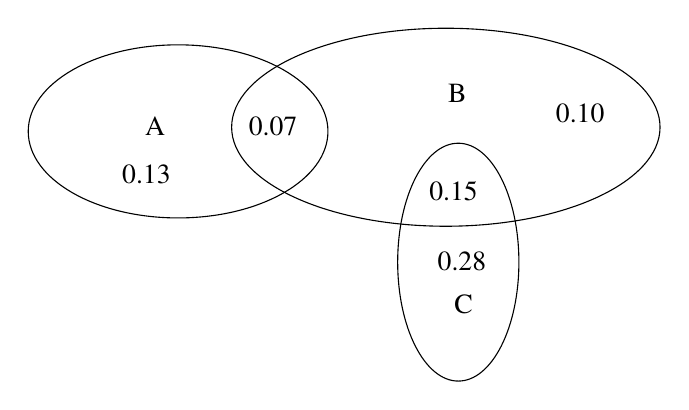
\begin{tikzpicture}[x=0.75pt,y=0.75pt,yscale=-1,xscale=1] 
 
\draw   (106,103.3) .. controls (106,80.27) and (138.33,61.6) .. (178.2,61.6) .. controls (218.07,61.6) and (250.4,80.27) .. (250.4,103.3) .. controls (250.4,126.33) and (218.07,145) .. (178.2,145) .. controls (138.33,145) and (106,126.33) .. (106,103.3) -- cycle ; 
\draw   (204,101.3) .. controls (204,74.96) and (250.2,53.6) .. (307.2,53.6) .. controls (364.2,53.6) and (410.4,74.96) .. (410.4,101.3) .. controls (410.4,127.64) and (364.2,149) .. (307.2,149) .. controls (250.2,149) and (204,127.64) .. (204,101.3) -- cycle ; 
\draw   (313.2,109) .. controls (329.33,109) and (342.4,134.65) .. (342.4,166.3) .. controls (342.4,197.95) and (329.33,223.6) .. (313.2,223.6) .. controls (297.07,223.6) and (284,197.95) .. (284,166.3) .. controls (284,134.65) and (297.07,109) .. (313.2,109) -- cycle ; 
 
\draw (161,95) node [anchor=north west][inner sep=0.75pt]   [align=left] {A}; 
\draw (307,79) node [anchor=north west][inner sep=0.75pt]   [align=left] {B}; 
\draw (310,181) node [anchor=north west][inner sep=0.75pt]   [align=left] {C}; 
\draw (150,118) node [anchor=north west][inner sep=0.75pt]   [align=left] {0.13}; 
\draw (211,95) node [anchor=north west][inner sep=0.75pt]   [align=left] {0.07}; 
\draw (298,126) node [anchor=north west][inner sep=0.75pt]   [align=left] {0.15}; 
\draw (359,89) node [anchor=north west][inner sep=0.75pt]   [align=left] {0.10}; 
\draw (302,160) node [anchor=north west][inner sep=0.75pt]   [align=left] {0.28\\}; 
 
 
\end{tikzpicture}

		\caption {generated by Latextikz}
		\label{fig:exemplar/11/16/3/11}
	\end{figure}
		\solution
		\iffalse
\documentclass[journal,11pt,onecolumn]{IEEEtran}
\usepackage{setspace}
\usepackage{gensymb}
\singlespacing
\usepackage[cmex10]{amsmath}
\usepackage{amsthm}
\usepackage{mathrsfs}
\usepackage{txfonts}
\usepackage{stfloats}
\usepackage{bm}
\usepackage{cite}
\usepackage{cases}
\usepackage{subfig}
\usepackage{longtable}
\usepackage{multirow}
\usepackage{enumitem}
\usepackage{mathtools}
\usepackage{tikz}
\usepackage{circuitikz}
\usepackage{verbatim}
\usepackage[breaklinks=true]{hyperref}
\usepackage{tkz-euclide} % loads  TikZ and tkz-base
\usepackage{listings}
\usepackage{color}    
\usepackage{array}    
\usepackage{longtable}
\usepackage{calc}     
\usepackage{multirow} 
\usepackage{hhline}   
\usepackage{ifthen}   
\usepackage{lscape}     
\usepackage{chngcntr}
\usepackage{float}
\DeclareMathOperator*{\Res}{Res}
\renewcommand\thesection{\arabic{section}}
\renewcommand\thesubsection{\thesection.\arabic{subsection}}
\renewcommand\thesubsubsection{\thesubsection.\arabic{subsubsection}}

\renewcommand\thesectiondis{\arabic{section}}
\renewcommand\thesubsectiondis{\thesectiondis.\arabic{subsection}}
\renewcommand\thesubsubsectiondis{\thesubsectiondis.\arabic{subsubsection}}
\renewcommand\thetable{\arabic{table}}
% correct bad hyphenation here
\hyphenation{op-tical net-works semi-conduc-tor}
\def\inputGnumericTable{}                                 %%

\lstset{
%language=C,
frame=single, 
breaklines=true,
columns=fullflexible
}
%\lstset{
%language=tex,
%frame=single, 
%breaklines=true
%}

\title{Assignment}
\author{Barath surya M | EE22BTECH11014}
\begin{document}
\newtheorem{theorem}{Theorem}[section]
\newtheorem{problem}{Problem}
\newtheorem{proposition}{Proposition}[section]
\newtheorem{lemma}{Lemma}[section]
\newtheorem{corollary}[theorem]{Corollary}
\newtheorem{example}{Example}[section]
\newtheorem{definition}[problem]{Definition}
\newcommand{\BEQA}{\begin{eqnarray}}
\newcommand{\EEQA}{\end{eqnarray}}
\newcommand{\define}{\stackrel{\triangle}{=}}
\bibliographystyle{IEEEtran}
\providecommand{\mbf}{\mathbf}
\providecommand{\pr}[1]{\ensuremath{\Pr\left(#1\right)}}
\providecommand{\qfunc}[1]{\ensuremath{Q\left(#1\right)}}
\providecommand{\sbrak}[1]{\ensuremath{{}\left[#1\right]}}
\providecommand{\lsbrak}[1]{\ensuremath{{}\left[#1\right.}}
\providecommand{\rsbrak}[1]{\ensuremath{{}\left.#1\right]}}
\providecommand{\brak}[1]{\ensuremath{\left(#1\right)}}
\providecommand{\lbrak}[1]{\ensuremath{\left(#1\right.}}
\providecommand{\rbrak}[1]{\ensuremath{\left.#1\right)}}
\providecommand{\cbrak}[1]{\ensuremath{\left\{#1\right\}}}
\providecommand{\lcbrak}[1]{\ensuremath{\left\{#1\right.}}
\providecommand{\rcbrak}[1]{\ensuremath{\left.#1\right\}}}
\theoremstyle{remark}
\newtheorem{rem}{Remark}
\newcommand{\sgn}{\mathop{\mathrm{sgn}}}
\providecommand{\abs}[1]{\left\vert#1\right\vert}
\providecommand{\res}[1]{\Res\displaylimits_{#1}} 
\providecommand{\norm}[1]{\left\lVert#1\right\rVert}
\providecommand{\mtx}[1]{\mathbf{#1}}
\providecommand{\mean}[1]{E\left[ #1 \right]}
\providecommand{\fourier}{\overset{\mathcal{F}}{ \rightleftharpoons}}
\providecommand{\system}[1]{\overset{\mathcal{#1}}{ \longleftrightarrow}}
\newcommand{\solution}{\noindent \textbf{Solution: }}
\newcommand{\cosec}{\,\text{cosec}\,}
\providecommand{\dec}[2]{\ensuremath{\overset{#1}{\underset{#2}{\gtrless}}}}
\newcommand{\myvec}[1]{\ensuremath{\begin{pmatrix}#1\end{pmatrix}}}
\newcommand{\mydet}[1]{\ensuremath{\begin{vmatrix}#1\end{vmatrix}}}
\let\vec\mathbf
\def\putbox#1#2#3{\makebox[0in][l]{\makebox[#1][l]{}\raisebox{\baselineskip}[0in][0in]{\raisebox{#2}[0in][0in]{#3}}}}
     \def\rightbox#1{\makebox[0in][r]{#1}}
     \def\centbox#1{\makebox[0in]{#1}}
     \def\topbox#1{\raisebox{-\baselineskip}[0in][0in]{#1}}
     \def\midbox#1{\raisebox{-0.5\baselineskip}[0in][0in]{#1}}
\maketitle
\vspace{3cm}
Question 11.16.3.11\\
The accompanying venn diagram shows three events, A, B and C, and also the probabilities of the various intersections (for instance, $\pr{AB}=0.7$. Determine 
\begin{enumerate}
	\item \pr{A}
	\item \pr{BC'}
	\item \pr{A+B}
	\item \pr{AB'}
	\item \pr{BC}
	\item \text{Probability of exactly one of the three occurs}
\end{enumerate}
\begin{figure}[h!]
	\centering
	\tikzset{every picture/.style={line width=0.75pt}}   
 
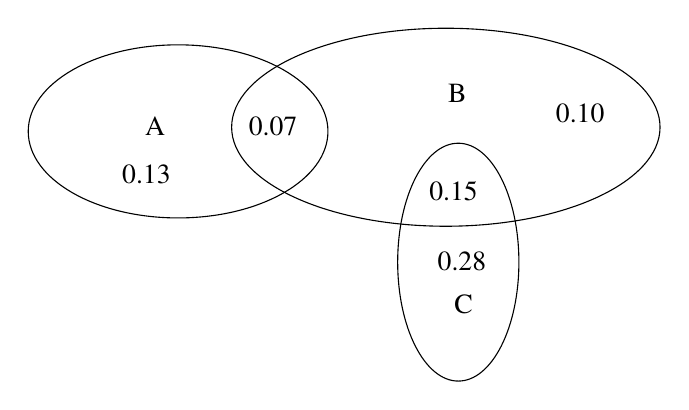
\begin{tikzpicture}[x=0.75pt,y=0.75pt,yscale=-1,xscale=1] 
 
\draw   (106,103.3) .. controls (106,80.27) and (138.33,61.6) .. (178.2,61.6) .. controls (218.07,61.6) and (250.4,80.27) .. (250.4,103.3) .. controls (250.4,126.33) and (218.07,145) .. (178.2,145) .. controls (138.33,145) and (106,126.33) .. (106,103.3) -- cycle ; 
\draw   (204,101.3) .. controls (204,74.96) and (250.2,53.6) .. (307.2,53.6) .. controls (364.2,53.6) and (410.4,74.96) .. (410.4,101.3) .. controls (410.4,127.64) and (364.2,149) .. (307.2,149) .. controls (250.2,149) and (204,127.64) .. (204,101.3) -- cycle ; 
\draw   (313.2,109) .. controls (329.33,109) and (342.4,134.65) .. (342.4,166.3) .. controls (342.4,197.95) and (329.33,223.6) .. (313.2,223.6) .. controls (297.07,223.6) and (284,197.95) .. (284,166.3) .. controls (284,134.65) and (297.07,109) .. (313.2,109) -- cycle ; 
 
\draw (161,95) node [anchor=north west][inner sep=0.75pt]   [align=left] {A}; 
\draw (307,79) node [anchor=north west][inner sep=0.75pt]   [align=left] {B}; 
\draw (310,181) node [anchor=north west][inner sep=0.75pt]   [align=left] {C}; 
\draw (150,118) node [anchor=north west][inner sep=0.75pt]   [align=left] {0.13}; 
\draw (211,95) node [anchor=north west][inner sep=0.75pt]   [align=left] {0.07}; 
\draw (298,126) node [anchor=north west][inner sep=0.75pt]   [align=left] {0.15}; 
\draw (359,89) node [anchor=north west][inner sep=0.75pt]   [align=left] {0.10}; 
\draw (302,160) node [anchor=north west][inner sep=0.75pt]   [align=left] {0.28\\}; 
 
 
\end{tikzpicture}

	\caption {generated by Latextikz}
	\label{fig:exemplar/11/16/3/11}
\end{figure}
\solution
\fi
Given:\\
From \figref{fig:exemplar/11/16/3/11}
\begin{align}
\pr{AB}=0.07\\
\pr{AB'}=0.13\\
\pr{BC}=0.15\\
\pr{BA'C'}=0.10\\
\pr{CB'}=0.28
\end{align}
\begin{enumerate}
\item \begin{align}
	\pr{A}&= 0.13+0.07\\
	&=0.2
	\end{align}
\item \begin{align}
	\pr{BC'} &=0.07+0.10+0.15-0.15\\
	&=0.17
\end{align}
\item \begin{align}
	\pr{A+B}&= \pr{A}+\pr{B} -\pr{AB}\\
	&=0.20+\brak{0.07+0.10+0.15}-0.07\\
	&=0.45
\end{align} 
\item \begin{align}
	\pr{AB'}&=0.20-0.07\\
	&=0.13
\end{align}
\item \begin{align}
	\pr{BC}&=0.15
\end{align} 
\item \begin{align}
	\pr{\text{AB'}} +\pr{CB'}+\pr{BA'C'} &= 0.13+0.10+0.28\\
	&=0.51
\end{align} 
\end{enumerate}


 

  
\item Events E and F are such that P(not E or not F) = 0.25, State whether E and F are
mutually exclusive.
\iffalse
\let\negmedspace\undefined
\let\negthickspace\undefined
\documentclass[article]{IEEEtran}
       \def\inputGnumericTable{}                                 %%
\usepackage{cite}
\usepackage{amsmath,amssymb,amsfonts,amsthm}
\usepackage{algorithmic}
\usepackage{graphicx}
\usepackage{textcomp}
\usepackage{xcolor}
\usepackage{txfonts}
\usepackage{listings}
\usepackage{enumitem}
\usepackage{mathtools}
\usepackage{gensymb}
\usepackage[breaklinks=true]{hyperref}
\usepackage{tkz-euclide} % loads  TikZ and tkz-base
\usepackage{listings}
%
%\usepackage{setspace}
%\usepackage{gensymb}
%\doublespacing
%\singlespacing

%\usepackage{graphicx}
%\usepackage{amssymb}
%\usepackage{relsize}
%\usepackage[cmex10]{amsmath}
%\usepackage{amsthm}
%\interdisplaylinepenalty=2500
%\savesymbol{iint}
%\usepackage{txfonts}
%\restoresymbol{TXF}{iint}
%\usepackage{wasysym}
%\usepackage{amsthm}
%\usepackage{iithtlc}
%\usepackage{mathrsfs}
%\usepackage{txfonts}
%\usepackage{stfloats}
%\usepackage{bm}
%\usepackage{cite}
%\usepackage{cases}
%\usepackage{subfig}
%\usepackage{xtab}
%\usepackage{longtable}
%\usepackage{multirow}
%\usepackage{algorithm}
%\usepackage{algpseudocode}
%\usepackage{enumitem}
%\usepackage{mathtools}
%\usepackage{tikz}
%\usepackage{circuitikz}
%\usepackage{verbatim}
%\usepackage{tfrupee}
%\usepackage{stmaryrd}
%\usetkzobj{all}
    \usepackage{color}                                            %%
    \usepackage{array}                                            %%
    \usepackage{longtable}                                        %%
    \usepackage{calc}                                             %%
    \usepackage{multirow}                                         %%
    \usepackage{hhline}                                           %%
    \usepackage{ifthen}                                           %%
 %optionally (for landscape tables embedded in another document): %%
    \usepackage{lscape}     
%\usepackage{multicol}
%\usepackage{chngcntr}
%\usepackage{enumerate}

%\usepackage{wasysym}
%\documentclass[conference]{IEEEtran}
%\IEEEoverridecommandlockouts
% The preceding line is only needed to identify funding in the first footnote. If that is unneeded, please comment it out.

\newtheorem{theorem}{Theorem}[section]
\newtheorem{problem}{Problem}
\newtheorem{proposition}{Proposition}[section]
\newtheorem{lemma}{Lemma}[section]
\newtheorem{corollary}[theorem]{Corollary}
\newtheorem{example}{Example}[section]
\newtheorem{definition}[problem]{Definition}
%\newtheorem{thm}{Theorem}[section] 
%\newtheorem{defn}[thm]{Definition}
%\newtheorem{algorithm}{Algorithm}[section]
%\newtheorem{cor}{Corollary}
\newcommand{\BEQA}{\begin{eqnarray}}
\newcommand{\EEQA}{\end{eqnarray}}
\newcommand{\define}{\stackrel{\triangle}{=}}
\theoremstyle{remark}
\newtheorem{rem}{Remark}

\begin{document}
\providecommand{\pr}[1]{\ensuremath{\Pr\left(#1\right)}}
\providecommand{\prt}[2]{\ensuremath{p_{#1}^{\left(#2\right)} }}        % own macro for this question
\providecommand{\qfunc}[1]{\ensuremath{Q\left(#1\right)}}
\providecommand{\sbrak}[1]{\ensuremath{{}\left[#1\right]}}
\providecommand{\lsbrak}[1]{\ensuremath{{}\left[#1\right.}}
\providecommand{\rsbrak}[1]{\ensuremath{{}\left.#1\right]}}
\providecommand{\brak}[1]{\ensuremath{\left(#1\right)}}
\providecommand{\lbrak}[1]{\ensuremath{\left(#1\right.}}
\providecommand{\rbrak}[1]{\ensuremath{\left.#1\right)}}
\providecommand{\cbrak}[1]{\ensuremath{\left\{#1\right\}}}
\providecommand{\lcbrak}[1]{\ensuremath{\left\{#1\right.}}
\providecommand{\rcbrak}[1]{\ensuremath{\left.#1\right\}}}
\newcommand{\sgn}{\mathop{\mathrm{sgn}}}
\providecommand{\abs}[1]{\left\vert#1\right\vert}
\providecommand{\res}[1]{\Res\displaylimits_{#1}} 
\providecommand{\norm}[1]{\left\lVert#1\right\rVert}
%\providecommand{\norm}[1]{\lVert#1\rVert}
\providecommand{\mtx}[1]{\mathbf{#1}}
\providecommand{\mean}[1]{E\left[ #1 \right]}
\providecommand{\cond}[2]{#1\middle|#2}
\providecommand{\fourier}{\overset{\mathcal{F}}{ \rightleftharpoons}}
\newenvironment{amatrix}[1]{%
  \left(\begin{array}{@{}*{#1}{c}|c@{}}
}{%
  \end{array}\right)
}
%\providecommand{\hilbert}{\overset{\mathcal{H}}{ \rightleftharpoons}}
%\providecommand{\system}{\overset{\mathcal{H}}{ \longleftrightarrow}}
	%\newcommand{\solution}[2]{\textbf{Solution:}{#1}}
\newcommand{\solution}{\noindent \textbf{Solution: }}
\newcommand{\cosec}{\,\text{cosec}\,}
\providecommand{\dec}[2]{\ensuremath{\overset{#1}{\underset{#2}{\gtrless}}}}
\newcommand{\myvec}[1]{\ensuremath{\begin{pmatrix}#1\end{pmatrix}}}
\newcommand{\mydet}[1]{\ensuremath{\begin{vmatrix}#1\end{vmatrix}}}
\newcommand{\myaugvec}[2]{\ensuremath{\begin{amatrix}{#1}#2\end{amatrix}}}
\providecommand{\rank}{\text{rank}}
\providecommand{\pr}[1]{\ensuremath{\Pr\left(#1\right)}}
\providecommand{\qfunc}[1]{\ensuremath{Q\left(#1\right)}}
	\newcommand*{\permcomb}[4][0mu]{{{}^{#3}\mkern#1#2_{#4}}}
\newcommand*{\perm}[1][-3mu]{\permcomb[#1]{P}}
\newcommand*{\comb}[1][-1mu]{\permcomb[#1]{C}}
\providecommand{\qfunc}[1]{\ensuremath{Q\left(#1\right)}}
\providecommand{\gauss}[2]{\mathcal{N}\ensuremath{\left(#1,#2\right)}}
\providecommand{\diff}[2]{\ensuremath{\frac{d{#1}}{d{#2}}}}
\providecommand{\myceil}[1]{\left \lceil #1 \right \rceil }
\newcommand\figref{Fig.~\ref}
\newcommand\tabref{Table~\ref}
\newcommand{\sinc}{\,\text{sinc}\,}
\newcommand{\rect}{\,\text{rect}\,}
%%
%	%\newcommand{\solution}[2]{\textbf{Solution:}{#1}}
%\newcommand{\solution}{\noindent \textbf{Solution: }}
%\newcommand{\cosec}{\,\text{cosec}\,}
%\numberwithin{equation}{section}
%\numberwithin{equation}{subsection}
%\numberwithin{problem}{section}
%\numberwithin{definition}{section}
%\makeatletter
%\@addtoreset{figure}{problem}
%\makeatother

%\let\StandardTheFigure\thefigure
\let\vec\mathbf

\bibliographystyle{IEEEtran}
\title{
%	\logo{
Assignment
%	}
}
\author{ Karthikeya hanu prakash kanithi (EE22BTECH11026)}
\maketitle

\vspace{3cm}
Question : Three dice are thrown at the sametime. Find the probability of getting three
two’s, if it is known that the sum of the numbers on the dice was six.
\fi
\\\solution 
Let $X_1, X_2, X_3$ be Bernoulli Random Variables as defined in  \autoref{tab:exemplar/12/13/3/14},
\begin{table}[h]
	\centering
	\input{exemplar/12/13/3/14/tables/Table2.tex}
	\caption{Random variable $X_i$ declaration $\forall i \in {1,2,3}$.}
        \label{tab:exemplar/12/13/3/14}
\end{table}
\\We need to find the value of
\begin{align}
\pr{X_1=2,X_2=2,X_3=2|X_1+X_2+X_3=6}
\end{align}
\\The pmf's of the random variables are as follows:
\begin{equation}
    p_{X_1}(k) = \label{eq:12/13/3/14}
    \begin{cases}
        \frac{1}{6} &  x \in \{1,2,3,4,5,6\} \\
        0 &  \text{otherwise}
    \end{cases}
\end{equation}
Now, If 
\begin{align}
X=X_1+X_2+X_3
\end{align}
Then
\begin{align}
      M_{X}(z)&=\prod_{i=1}^{3}M_{X_i}(z)\\
      &= \prod_{i=1}^{3}\left(\sum_{k=1}^{6} \frac{z^{-k}}{6}\right) \label{eq:12/13/3/14/3}\\
      &= \frac{z^{-3}}{216} + \frac{3z^{-4}}{216} + \frac{6z^{-5}}{216} + \frac{10z^{-6}}{216} + \ldots 
\end{align}
From \eqref{eq:12/13/3/14}, When all the three die's roll 2, then thier sum will be 6. So, 
\begin{align}
&\pr{X_1=X_2=X_3=2 ,\ X_1+X_2+X_3=6} \label{eq:12/13/3/14/4} \\ 
&= p_{X_1}(2) p_{X_2}(2) p_{X_3}(2)
= \left(\frac{1}{6}\right)^3
= \frac{1}{216}
\end{align}
From \eqref{eq:12/13/3/14/3}, the probability that the sum of all three die's is 6 is,
\begin{align}
\pr{X_1+X_2+X_3=6} &= \frac{10}{216} \label{eq:12/13/3/14/5}
\end{align}
From \eqref{eq:12/13/3/14/4} and \eqref{eq:12/13/3/14/5}, the probability of getting three two’s, if it is known that the sum of the numbers on the dice was six will be
\begin{align}
&\pr{X_1=2,X_2=2,X_3=2|X_1+X_2+X_3=6} \\ 
&= \frac{\pr{X_1=X_2=X_3=2 ,\ X_1+X_2+X_3=6}}{\pr{X_1+X_2+X_3=6}}\\
&= \frac{\frac{1}{216}}{\frac{10}{216}}
=\frac{1}{10}
\end{align}






















\item State whether the statement is True or False.\\
The probability that a person visiting a zoo will see the giraffe is 0.72, the probability that he will see the bears is 0.84 and the probability that he will see both is 0.52.\\
\solution
\\
\iffalse
\let\negmedspace\undefined
\let\negthickspace\undefined
\documentclass[journal,12pt,onecolumn]{IEEEtran}
\usepackage{cite}
\usepackage{amsmath,amssymb,amsfonts,amsthm}
\usepackage{algorithmic}
\usepackage{graphicx}
\usepackage{textcomp}
\usepackage{xcolor}
\usepackage{txfonts}
\usepackage{listings}
\usepackage{enumitem}
\usepackage{mathtools}
\usepackage{gensymb}
\usepackage{comment}
\usepackage[breaklinks=true]{hyperref}
\usepackage{tkz-euclide} 
\usepackage{listings}
\usepackage{gvv}                                        
\def\inputGnumericTable{}                                 
\usepackage[latin1]{inputenc}                                
\usepackage{color}                                            
\usepackage{array}                                            
\usepackage{longtable}                                       
\usepackage{calc}                                             
\usepackage{multirow}                                         
\usepackage{hhline}                                           
\usepackage{ifthen}                                           
\usepackage{lscape}

\newtheorem{theorem}{Theorem}[section]
\newtheorem{problem}{Problem}
\newtheorem{proposition}{Proposition}[section]
\newtheorem{lemma}{Lemma}[section]
\newtheorem{corollary}[theorem]{Corollary}
\newtheorem{example}{Example}[section]
\newtheorem{definition}[problem]{Definition}
\newcommand{\BEQA}{\begin{eqnarray}}
\newcommand{\EEQA}{\end{eqnarray}}
\newcommand{\define}{\stackrel{\triangle}{=}}
\theoremstyle{remark}
\newtheorem{rem}{Remark}
\begin{document}

\bibliographystyle{IEEEtran}
\vspace{3cm}


\title{Question 12.13.3.18}
\author{EE22BTECH11051}

\maketitle
\vspace{3cm}

\textbf{Question:} A box has 5 blue and 4 red balls. One ball is drawn at random and not replaced.
Its colour is also not noted. Then another ball is drawn at random. What is the
probability of second ball being blue?

\textbf{Solution:} \\
\fi
Let X and Y denote the random variables for the first and second draw respectively as follows:
\begin{table}[h]
    \centering
    %%%%%%%%%%%%%%%%%%%%%%%%%%%%%%%%%%%%%%%%%%%%%%%%%%%%%%%%%%%%%%%%%%%%%%
%%                                                                  %%
%%  This is a LaTeX2e table fragment exported from Gnumeric.        %%
%%                                                                  %%
%%%%%%%%%%%%%%%%%%%%%%%%%%%%%%%%%%%%%%%%%%%%%%%%%%%%%%%%%%%%%%%%%%%%%%

\begin{center}
    \begin{tabular}{|c|c|c|}
    \hline
    \textbf{RV}& \textbf{Values} & \textbf{Description} \\ \hline
    $X$		   & 	$\{0,1\}$	&  1st draw :- 0: blue, 1: red\\ \hline
    $Y$ 		   & 	$\{0,1\}$	&  2nd draw :- 0: blue, 1: red\\ \hline
    \end{tabular}
    \end{center}
    \caption{Random Variables}
    \label{12.13.3.8_table_1}
    \end{table}
\\
The probabilities are given as:
\begin{align}
    \pr{X = 0} = \frac{5}{9}\\
    \pr{X = 1} = \frac{4}{9}
\end{align}
\begin{align}
    \pr{Y = 0 | X = 0} = \frac{\pr{Y = 0,X = 0}}{\pr{X = 0}} = \frac{1}{2}\\
    \pr{Y = 0 | X = 1} = \frac{\pr{Y = 0,X = 1}}{\pr{X = 1}} = \frac{5}{8}
\end{align}
    \\
The probability of the second ball beign drawn being blue is given as:
\begin{align}
\pr{Y = 0} &= \pr{X = 0}\pr{Y = 0 | X = 0} + \pr{X = 1}\pr{Y = 0 | X = 1}\\
           &= {\frac{5}{9}}\times{\frac{1}{2}} + {\frac{4}{9}}\times{{\frac{5}{8}}}\\
           &= \frac{5}{9}
\end{align}

\end{enumerate}
